\documentclass{article}
\usepackage{tikz}

\begin{document}

Hello, World!

This is a test document for TeXpresso.

\section{Introduction}
LaTeX is a document preparation system.

\subsection{Mathematics}
Inline math: $E = mc^2$

Display math:
\begin{equation}
  \int_0^\infty e^{-x^2} dx = \frac{\sqrt{\pi}}{2}
\end{equation}

\subsection{TikZ Graphics}
Here is a simple TikZ drawing:

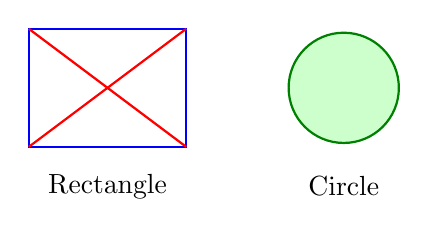
\begin{tikzpicture}
  % A simple shape
  \draw[thick, blue] (0,0) rectangle (2,1.5);
  \draw[thick, red] (0,0) -- (2,1.5);
  \draw[thick, red] (2,0) -- (0,1.5);

  % A circle
  \draw[thick, green!50!black, fill=green!20] (4,0.75) circle (0.7);

  % Some text
  \node at (1, -0.5) {Rectangle};
  \node at (4, -0.5) {Circle};
\end{tikzpicture}

\end{document}
